\documentclass[12pt]{article}

\usepackage[english]{babel}

% Math/Greek packages
\usepackage{amssymb,amsmath,amsthm, mathtools} 
\usepackage{algorithm, algorithmic}
\usepackage{upgreek, siunitx}

% Graphics/Presentation packages
\usepackage{geometry, graphicx}
\usepackage{tabulary, enumitem, array}
\usepackage{xparse,mleftright,tikz}
\usepackage{physics}

% Misc packages
\usepackage{fancyhdr}


\usepackage[export]{adjustbox}

\usepackage{esint}

\sisetup{locale=US,group-separator = {,}}
\usepackage[colorlinks=true, allcolors=blue]{hyperref}


% Box function - update this as more sophisticated solutions are found
\newcommand\mybox[2][]{\tikz[overlay]\node[fill=blue!20,inner sep=2pt, anchor=text, rectangle, rounded corners=1mm,#1] {#2};\phantom{#2}}
\renewcommand{\arraystretch}{1.2}

% General macro declarations


\makeatletter
\let\oldabs\abs
\def\abs{\@ifstar{\oldabs}{\oldabs*}}
%
\let\oldnorm\norm
\def\norm{\@ifstar{\oldnorm}{\oldnorm*}}
\makeatother

\begin{document}

\title{PHSX 461: HW09}
\author{William Jardee}
\maketitle

\section*{Question 1}
\emph{In strong coupling, the quantum states of photons ‘hybridize’ with the quantum states of electronic excitations (‘excitons’) in a material to form a superposition of light and matter quantum states (wow!). A crucial part of demonstrating this hybridization is to show “anti-crossing” behavior in the system. Let’s work it out here.}

\emph{the strong-coupling Hamiltonian is simplified to a two-level system composed of a photon state $(\ket{\text{photon}})$ and an exciton state $(\ket{\text{exciton}})$. the energy of the photon depends upon its wavelength: $E_p(\lambda)=(h c)/\lambda$(this is called dispersion). For the exciton, the energy is a constant, $E_x$. the strength of the coupling is usually referred to as $\Omega$ (assume it is real and positive). The quantum system then can be formulated as follows:}
\[\ket{\text{photon}} \rightarrow \vb{v}_1 = \mqty(1 \\ 0) \quad \ket{\text{photon}} \rightarrow \vb{v}_1 = \mqty(0 \\ 1) \quad \hat{H} \rightarrow H = \mqty(E_p(\lambda) & \Omega \\ \Omega & E_x)\]

\begin{enumerate}[label=\alph*)]
\item \emph{Determine allowed energies of the system (don't worry about the eigenvectors) in terms of $E_p(\lambda), E_x,$ and $\omega$. Call the larger energy $E_+$ and the lower energy $E_-$. Note that both depend on $\lambda$.}

\[H\vb{v} = E \vb{v}\]
Where $\vb{v}$ is an eigenstate of the system. 
\[0 = det\mqty|E_p(\lambda) -E & \Omega \\ \Omega & E_x - E|\]
\[(E_p(\lambda) - E)(E_x-E) - \Omega^2 = 0\]
\[E^2 - E(E_p(\lambda) + E_x) + E_p(\lambda)E_x - \Omega^2 = 0\]
Using the quadratic formula to solve this:
\[E = \frac{(E_p(\lambda) + E_x) \pm \sqrt{(E_p(\lambda)+E_x)^2 - 4((E_p(\lambda)+ E_x) - \Omega^2)}}{2}\]
\[ = \frac{(E_p(\lambda)+ E_x) \pm \sqrt{(E_p(\lambda))^2 + 2(E_p(\lambda)E_x) + E_x^2 - 4(E_p(\lambda)+ E_x - \Omega^2)}}{2}\]
\[= \frac{(E_p(\lambda)+ E_x) \pm \sqrt{(E_p(\lambda))^2 + E_x^2 -2(E_p(\lambda) + E_x) + 4\Omega^2}}{2}\]
\[= \frac{1}{2}(E_p(\lambda)+ E_x) \pm \sqrt{\Big(\frac{E_p(\lambda) - E_x}{2}\Big)^2 + \Omega^2}\]
From this, we get that the eigenstates of the Hamiltonian, and thus the possible energy values, is:
\[\boxed{E_+ = \frac{1}{2}(E_p(\lambda)+ E_x) + \sqrt{\Big(\frac{E_p(\lambda) - E_x}{2}\Big)^2 + \Omega^2}}\]
\[\boxed{E_- = \frac{1}{2}(E_p(\lambda)+ E_x) - \sqrt{\Big(\frac{E_p(\lambda) - E_x}{2}\Big)^2 + \Omega^2}}\]

\item \emph{Assume $E_x = 2.0$eV and $\Omega=0.005$eV. Use your favorite plotting software to plot on $E_+(\lambda)$ and $E_-(\lambda)$ over the range $500$nm$\leq \lambda \leq 700$nm on the same plot}\footnote{\textbf{Recall:} $h c = 1240$eV$\cdot$nm}

\begin{figure}[!ht]
\centering
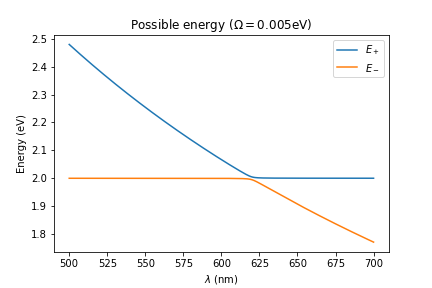
\includegraphics[width=0.60\textwidth]{./hw09_1.png}
\label{fig:1_1}
\end{figure}

\item \emph{Make a second plot that plots the energies of the energies of the exciton $(E_x)$ and $E_p(\lambda)$ over the same range when $\Omega = 0$ and there is no coupling between the states.}

\begin{figure}[!ht]
\centering
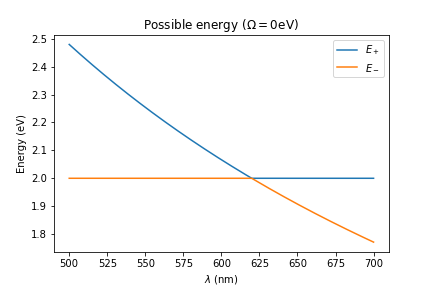
\includegraphics[width=0.60\textwidth]{./hw09_2.png}
\label{fig:1_2}
\end{figure}
\end{enumerate}

Notice how in (c) the energies of the exciton and photon intersect when there is no coupling where as in (b) the energies $E_+(\lambda)$ and $E_-(\lambda)$ never intersect when there is coupling! This ``avoided crossing" or ``anti-crossing" of the levels is characteritic of coupled systems. Note that the minimum separation between the two states is $\Omega$ (this splitting is referred to as the `Rabi splitting'). Mohammad, out TA, is working on this very subject right now! 

Final note, at $\lambda = 500$nm the $\ket{-}$ state is said to be ``exiton-like" and the $\ket{+}$ state is said the be ``photon-like" because the superpositions at this energy where $E_p \neq E_x$ are heavily waited to the $\ket{\text{exciton}}$ and $\ket{\text{photon}}$ states, respectively. In contrast, when $E_p = E_x$ the $\ket{-}$ and $\ket{+}$ states are superpositions of equal parts of the $\ket{\text{exciton}}$ and $\ket{\text{photon}}$ states. Work it out if you would like! 
\bigskip

This is pretty easy to see from the calculations of $E_+$ and $E_-$, as when they are equal the part that differs (the square root) simplifies as: $\sqrt{\Omega^2} = \Omega$. This kinda makes sense, as there is nothing to create a bias in if the state should be the $(\ket{\text{photon}})$ state of the $(\ket{\text{exciton}})$ state. Where when they are not equal, the difference will be nonzero. 

%--------------------------------------------------------------
\newpage

\section*{Griffiths 3.39}
\emph{$($no integrals allowed - seriously! use Dirac notation$)$}

Oh gosh, you're really gonna be testing my patience with the physics package...

\begin{itemize}
\item \emph{Find the expressions for $\hat{x}$ and $\hat{p}$ matrix elements}
Before we get too far into this, let's remind outselves of a couple vital things:
\[\hat{a}_+ \psi_n = \sqrt{n+1}\psi_{n+1} \qquad \hat{a}_- \psi_n = \sqrt{n}\psi_{n-1}\]
\[\hat{x} = i\sqrt{\frac{\hbar}{2m\omega}}\, (\hat{a}_+ + \hat{a}_-) \qquad \hat{p} = \sqrt{\frac{\hbar m \omega}{2}}\, (\hat{a}_+ - \hat{a}_-)\]

Now we can move onto the meat of the problem, first with $\hat{x}$:
\[\hat{x} = \mel**{\psi_n}{\sqrt{\frac{\hbar}{2m\omega}}\, (\hat{a}_+ + \hat{a}_-)}{\psi_{n^\prime}}\]
\[= \sqrt{\frac{\hbar}{2m\omega}} \mel{\psi_n}{\hat{a}_+ + \hat{a}_-}{\psi_{n^\prime}}\]
\[= \sqrt{\frac{\hbar}{2m\omega}} \Big[\mel{\psi_n}{\hat{a}_+}{\psi_{n^\prime}} + \mel{\psi_n}{\hat{a}_-}{\psi_{n^\prime}}\Big]\]
\[= \sqrt{\frac{\hbar}{2m\omega}}\Big[\braket{\hat{a}_- \psi_n}{\psi_{n^\prime}} + \braket{\psi_n}{\hat{a}_- \psi_{n^\prime}}\Big]\]
\[= \sqrt{\frac{\hbar}{2m\omega}}\Big[\sqrt{n}\braket{\psi_{n-1}}{\psi_{n^\prime}} + \sqrt{n^\prime}\braket{\psi_n}{\psi_{n^\prime - 1}}\Big]\]
\[\boxed{\hat{x}= \sqrt{\frac{\hbar}{2m\omega}}\Big[\sqrt{n}\, \delta_{n-1, n^\prime} + \sqrt{n^\prime}\, \delta_{n, n^\prime-1}\Big]}\]

Following a similar derivation for $\hat{p}$:

\[\hat{p} = \mel**{\psi_n}{i\sqrt{\frac{\hbar m \omega}{2}}\, (\hat{a}_+ + \hat{a}_-)}{\psi_{n^\prime}}\]
\[= i\sqrt{\frac{\hbar m \omega}{2}} \mel{\psi_n}{\hat{a}_+ - \hat{a}_-}{\psi_{n^\prime}}\]
\[= i\sqrt{\frac{\hbar m \omega}{2}} \Big[\mel{\psi_n}{\hat{a}_+}{\psi_{n^\prime}} - \mel{\psi_n}{\hat{a}_-}{\psi_{n^\prime}}\Big]\]
\[= i\sqrt{\frac{\hbar m \omega}{2}}\Big[\braket{\hat{a}_- \psi_n}{\psi_{n^\prime}} - \braket{\psi_n}{\hat{a}_- \psi_{n^\prime}}\Big]\]
\[= i\sqrt{\frac{\hbar m \omega}{2}}\Big[\sqrt{n}\braket{\psi_{n-1}}{\psi_{n^\prime}} - \sqrt{n^\prime}\braket{\psi_n}{\psi_{n^\prime - 1}}\Big]\]
\[\boxed{\hat{p}= i\sqrt{\frac{\hbar m \omega}{2}}\Big[\sqrt{n}\, \delta_{n-1, n^\prime} - \sqrt{n^\prime}\, \delta_{n, n^\prime-1}\Big]}\]



\item \emph{For each operator, draw a representation of the infinite-dimensional matrix that is described by the expressions above. Describe all zero and non-zero regions of the matrix}

\[\hat{x} \Longrightarrow \sqrt{\frac{\hbar}{2m\omega}} \mqty[0 & 1 & 0 & 0 & \cdots \\ 1 & 0 & \sqrt{2} & 0 & \cdots \\ 0 & \sqrt{2} & 0 & \sqrt{3} & \cdots \\ 0 & 0 & \sqrt{3} & 0 & \cdots \\ \cdots & \cdots & \cdots & \cdots & \cdots]\]


\[\hat{p} \Longrightarrow i\sqrt{\frac{\hbar}{2m\omega}} \mqty[0 & -1 & 0 & 0 & \cdots \\ 1 & 0 & -\sqrt{2} & 0 & \cdots \\ 0 & \sqrt{2} & 0 & -\sqrt{3} & \cdots \\ 0 & 0 & \sqrt{3} & 0 & \cdots \\ \cdots & \cdots & \cdots & \cdots & \cdots]\]

\item \emph{Show that $(1/2m)P^2 + (m\omega^2 /2)X^2 = H$}\footnote{I wasn't sure if we were supposed to do this part too, so I did. Good practice either way.}

First we must get the $\hat{x}^2$ and $\hat{p}^2$ matrices:
\[\mel{\psi_n}{\hat{p}^2}{\psi_{n^\prime}} = -\frac{\hbar m \omega}{2}\mel{\psi_n}{(\hat{a}_+ - \hat{a}_-)^2}{\psi_{n^\prime}}\]
\[= -\frac{\hbar m \omega}{2}\Big[\braket{\psi_n}{\hat{a}_+\hat{a}_+ \psi_{n^\prime}} - \braket{\psi_n}{\hat{a}_+\hat{a}_- \psi_{n^\prime}} - \braket{\psi_n}{\hat{a}_-\hat{a}_+ \psi_{n^\prime}} + \braket{\psi_n}{\hat{a}_-\hat{a}_- \psi_{n^\prime}}\Big]\]

\[= -\frac{\hbar m \omega}{2}\Big[\braket{\psi_n}{\sqrt{n^\prime + 1}\sqrt{n^\prime + 2} \psi_{n^\prime+2}} - \braket{\psi_n}{\sqrt{n^\prime}\sqrt{n^\prime} \psi_{n^\prime}}\]
\[- \braket{\psi_n}{\sqrt{n^\prime + 1}\sqrt{n^\prime + 1} \psi_{n^\prime}} + \braket{\psi_n}{\sqrt{n^\prime}\sqrt{n^\prime -1} \psi_{n^\prime-2}}\Big]\]

\[= -\frac{\hbar m \omega}{2}\Big[
\sqrt{n^\prime + 1}\sqrt{n^\prime + 2} \, \delta_{n, n^\prime +2} 
- (2n^\prime + 1) \, \delta_{n, n^\prime} 
+ \sqrt{n^\prime}\sqrt{n^\prime -1} \, \delta_{n, n^\prime -2}\Big]\]

\[\hat{p}^2 \Longrightarrow \frac{\hbar m \omega}{2} \mqty[
1 & 0 & -\sqrt{1 \cdot 2} & 0 & \cdots \\ 
0 & 3 & 0 & -\sqrt{2 \cdot 3} & \cdots \\ 
-\sqrt{1 \cdot 2} & 0 & 5 & 0 & \cdots \\ 
0 & -\sqrt{2 \cdot 3} & 0 & 7 & \cdots \\ 
\cdots & \cdots & \cdots & \cdots & \cdots]\]

Through a very similar derivation, there is a: 
\[\hat{x}^2 \Longrightarrow \frac{\hbar}{2m \omega} \mqty[
1 & 0 & \sqrt{1 \cdot 2} & 0 & \cdots \\ 
0 & 3 & 0 & \sqrt{2 \cdot 3} & \cdots \\ 
\sqrt{1 \cdot 2} & 0 & 5 & 0 & \cdots \\ 
0 & \sqrt{2 \cdot 3} & 0 & 7 & \cdots \\ 
\cdots & \cdots & \cdots & \cdots & \cdots]\]

So, plugging these into the equation $(1/2m)P^2 + (m\omega^2 /2)X^2 = H$:
\[\frac{1}{2m}\frac{\hbar m \omega}{2} \mqty[
1 & 0 & -\sqrt{1 \cdot 2} & 0 & \cdots \\ 
0 & 3 & 0 & -\sqrt{2 \cdot 3} & \cdots \\ 
-\sqrt{1 \cdot 2} & 0 & 5 & 0 & \cdots \\ 
0 & -\sqrt{2 \cdot 3} & 0 & 7 & \cdots \\ 
\cdots & \cdots & \cdots & \cdots & \cdots] \]
\[+ \frac{m \omega^2}{2}
\frac{\hbar}{2m \omega} \mqty[
1 & 0 & \sqrt{1 \cdot 2} & 0 & \cdots \\ 
0 & 3 & 0 & \sqrt{2 \cdot 3} & \cdots \\ 
\sqrt{1 \cdot 2} & 0 & 5 & 0 & \cdots \\ 
0 & \sqrt{2 \cdot 3} & 0 & 7 & \cdots \\ 
\cdots & \cdots & \cdots & \cdots & \cdots]\]
\[= \frac{\hbar \omega}{2} \mqty[
1 & 0 & 0 & 0 & \cdots \\ 
0 & 3 & 0 & 0 & \cdots \\ 
0 & 0 & 5 & 0 & \cdots \\ 
0 & 0 & 0 & 7 & \cdots \\ 
\cdots & \cdots & \cdots & \cdots & \cdots]\]
Does this correspond to $\hat{H}$?
\[\mel{\psi_n}{\hat{H}}{\psi_{n^\prime}}\]
\[= \braket{\psi_n}{\hat{H}\psi_{n^\prime}}\]
\[= \braket{\psi_n}{E_{n^\prime}\psi_{n^\prime}}\]
\[= E_{n^\prime}\braket{\psi_n}{\psi_{n^\prime}}\]
\[= E_{n^\prime}\, \delta_{n, n^\prime}\]
When we remember that $E_n = \hbar \omega (n + \frac{1}{2})$ for the QHO: 
\[\mel{\psi_n}{\hat{H}}{\psi_{n^\prime}} = \frac{\hbar \omega}{2} \mqty[
1 & 0 & 0 & 0 & \cdots \\ 
0 & 3 & 0 & 0 & \cdots \\ 
0 & 0 & 5 & 0 & \cdots \\ 
0 & 0 & 0 & 7 & \cdots \\ 
\cdots & \cdots & \cdots & \cdots & \cdots] \]
So, it would seem that $(1/2m)P^2 + (m\omega^2 /2)X^2 = H$ is satisfied.
\end{itemize}

%--------------------------------------------------------------
\newpage

\section*{Question 3}
\emph{A particle in a 1D QHO is in the state $\ket{\alpha} = \beta(\ket{0} - 3\ket{1} - 2i\ket{3})$ where $\ket{n}$ is the $n^\text{th}$ stationary state of the !D QHO at time $t=0$.
Consider these operators:}
\[\hat{Q} = \hbar \omega \sum_{n=0}^\infty \frac{2n+1}{2}(\ket{n}\bra{n}) \quad \hat{A} = \sum_{n=0}^\infty \sqrt{n+1}(\ket{n+1}\bra{n}) \quad \hat{B}=\sum_{n=0}^\infty \sqrt{n}(\ket{n-1}\bra{n})\]

\begin{enumerate}[label=\alph*)]
\item \emph{Calculate $\beta$}

To calculate $\beta$, let's first note that
\[\bra{\alpha} = \beta^* (\bra{0} - 3\bra{1} + 2i \bra{3})\]
So, now we can enforce the normalization constraint, that is
\[\braket{\alpha}{\alpha} = 1\]

\[1 = \beta^* (\bra{0} - 3\bra{1} + 2i \bra{3})\beta(\ket{0} - 3\ket{1} - 2i\ket{3})\]
\[1 = |\beta|^2 (\braket{0}{0} + 9\braket{1}{1} + 4\braket{3}{3})\]
\[1 = |\beta|^2 (14)\]
\[\boxed{\beta = \frac{1}{\sqrt{14}}}\]

\item \emph{Find the $\ev{Q}$. What is another name for $\hat{Q}$?}
\[\ev{Q} = \ev{\hat{Q}}{\alpha}\]
\[= \bra{\alpha}\hbar \omega \sum_{n=0}^\infty \frac{2n+1}{2}\ket{n}\braket{n}{\alpha}\]
\[\boxed{\ev{Q}=\frac{\hbar \omega}{2}(1+3+7)\Big(\frac{1}{14}\Big) = \frac{\hbar \omega}{2}\Big(\frac{11}{14}\Big)}\]

$\hat{Q}$ is just the Hamiltonian.

\item \emph{Calculate $\hat{A}\ket{\alpha}$. What is another name for $\hat{A}$?}
\[\hat{A}\ket{\alpha} = \sum_{n=0}^\infty \sqrt{n+1}\ket{n+1}\braket{n}{\alpha}\]
\[= \frac{1}{\sqrt{14}}\sum_{n=0}^\infty \sqrt{n+1} \ket{n+1}\bra{n}(\ket{0} - 3\ket{1} - 2i\ket{3})\]
\[= \frac{1}{\sqrt{14}}(\sqrt{1}\ket{1} - 3\sqrt{2}\ket{2} - \sqrt{4}2i \ket{4})\]
\[\boxed{\hat{A}\ket{\alpha}= \frac{1}{\sqrt{14}}(\ket{1} - 3\sqrt{2}\ket{2} - 4i \ket{4})}\]

$\hat{Q}$ is just the $\hat{a}_+$.


\item \emph{Calculate $\hat{B}\ket{\alpha}$. What is another name for $\hat{B}$?}

\[\hat{B}\ket{\alpha} = \sum_{n=0}^\infty \sqrt{n}\ket{n-1}\braket{n}{\alpha}\]
\[= \frac{1}{\sqrt{14}}\sum_{n=0}^\infty \sqrt{n}\ket{n-1}\bra{n}(\ket{0} - 3\ket{1} - 2i\ket{3})\]
\[= \frac{1}{\sqrt{14}}(\sqrt{0}\ket{-1} - 3\sqrt{1}\ket{0} - \sqrt{3}2i \ket{2})\]
\[\boxed{\hat{B}\ket{\alpha}= \frac{1}{\sqrt{14}}(- 3\ket{0} - 2\sqrt{3}i \ket{2})}\]

$\hat{Q}$ is just the $\hat{a}_-$.
\end{enumerate}

%--------------------------------------------------------------
\newpage

\section*{Griffiths 3.44 (b)}
\emph{\textbf{Note:} remember that to construct $\ket{S(t)}$ you need to multiply each eigenstate in of $\hat{H}$ that makes up the superposition of $\ket{S(0)}$ by the correct wiggle factor. Same stuff as earlier in the semester, now just with matrix representations of $\hat{H}$ and vectors for the states!}
\bigskip

\emph{The Hamiltonian for a certain three-level system is represended by the matrix}
\[H = \mqty[a&0&b\\0&c&0\\b&0&a]\]
\emph{where $a$, $b$, and $c$ are real numbers.}

\begin{enumerate}[label=\alph*)]
\item \emph{if the system starts out in the state}
\[\ket{S(0)} = \mqty(0\\1\\0)\]
\emph{what is $\ket{S(t)}$}\bigskip

Since $\ket{S(0)}$ is an eigenstate of $H$ with eigenvalue $c$, $\ket{S(0)}$ won't evolve in time except for with a ``wiggle factor":
\[\boxed{\ket{S(t)} = \ket{S(0)} e^{c \, t/ \hbar}}\]

\item \emph{if the system starts out in the state}
\[\ket{S(0)} = \mqty(1\\0\\0)\]
\emph{what is $\ket{S(t)}$}\bigskip

Since $\ket{S(0)}$ is not an eigenvector of $H$, we must find what linear combination of eigenvectors make it up. By looking back at a), we already have one of the eigenvectors. And, by educated guess (from the amount of symmetry in the problem), we can also say that 
\[\vb{v}_2 = \mqty(1\\0\\1) \qquad \vb{v}_3 = \mqty(1\\0\\-1)\]
are eigenvectors. To show this is true, let's multiply them out.
\[\mqty[a&0&b\\0&c&0\\b&0&a]\mqty(1\\0\\1) = \mqty(a+b\\0\\a+b) = (a+b)\mqty(1\\0\\1)\]
\[\mqty[a&0&b\\0&c&0\\b&0&a]\mqty(1\\0\\-1) = \mqty(0\\0\\0) = 0 \cdot \mqty(1\\0\\-1)\]

Conveniently, that also gave the eigenvalues. So, decomposing $\ket{S(0)}$ and applying the ``wiggle factor":
\[\ket{S(0)} = \mqty(1\\0\\0) = \frac{1}{2}\Big(\mqty(1\\0\\1) + \mqty(1\\0\\-1)\Big)\]
\[\ket{S(t)}= \frac{1}{2}\Big(\mqty(1\\0\\1) e^{(a+b) \, t/ \hbar}+ \mqty(1\\0\\-1)e^{0 \cdot \, t/ \hbar}\Big)\]
\[\boxed{\ket{S(t)} = \frac{1}{2}\Big(\mqty(1\\0\\1) e^{(a+b) \, t/ \hbar}+ \mqty(1\\0\\-1)\Big)}\]
\end{enumerate}

%--------------------------------------------------------------
\newpage


\section*{Griffiths 3.14 (a) and (b)}

\begin{enumerate}[label=\alph*)]
\item \emph{Prove the commutator identities}
\[\comm{\hat{A}+\hat{B}}{\hat{C}}\]
\[= (\hat{A}+\hat{B})(\hat{C}) - (\hat{C})(\hat{A} + \hat{B})\]
\[= \hat{A}\hat{C} + \hat{B}\hat{C} - \hat{C}\hat{A} - \hat{C}\hat{B}\]
\[= (\hat{A}\hat{C} - \hat{C}\hat{A}) + (\hat{B}\hat{C}-\hat{C}\hat{B})\]
\[\boxed{\comm{\hat{A}+\hat{B}}{\hat{C}}= \comm{\hat{A}}{\hat{C}} + \comm{\hat{B}}{\hat{C}}}\]
\bigskip

\[\comm{\hat{A}\hat{B}}{\hat{C}} = \hat{A}\hat{B}\hat{C} - \hat{C}\hat{A}\hat{B}\]
Perhaps this one is easier going the other direction
\[\hat{A}\comm{\hat{B}}{\hat{C}} + \comm{\hat{A}}{\hat{C}}\hat{B}\]
\[= \hat{A}(\hat{B}\hat{C}-\hat{C}\hat{B}) + (\hat{A}\hat{C}-\hat{C}\hat{A})\hat{B}\]
\[=\hat{A}\hat{B}\hat{C} - \hat{A}\hat{C}\hat{B} + \hat{A}\hat{C}\hat{B} - \hat{C}\hat{A}\hat{B}\]
\[ = \hat{A}\hat{B}\hat{C} - \hat{C}\hat{A}\hat{B}\]
\[\boxed{\hat{A}\comm{\hat{B}}{\hat{C}} + \comm{\hat{A}}{\hat{C}}\hat{B} = \comm{\hat{A}\hat{B}}{\hat{C}}}\]

\item \emph{Show that}
\[\comm{x^n}{\hat{p}} = i \hbar n x^{n-1}\]\bigskip

Recall that $\hat{p} = -i \hbar \pdv{x}$
\[\comm{x^n}{\hat{p}} = x^n \hat{p} - \hat{p}x^n\]
\[= x^n \hat{p}\cdot 1 - \hat{p}x^n\]
\[= x^n -i \hbar \pdv{x} 1 - \Big(-i \hbar \pdv{x}\Big)x^n\]
\[=0 + i\hbar n x^{n-1}\]
\[\boxed{\comm{x^n}{\hat{p}} = i\hbar n x^{n-1}}\]

\end{enumerate}

\end{document}